%% by Philipp.Schneider@ifp.uni-stuttgart.de
%% 17.01.22 Created

\documentclass[a4paper,twoside]{book}%[draft]
\usepackage[a4paper]{geometry}

\usepackage{etoolbox}
\patchcmd{\chapter}{\thispagestyle{plain}}{\thispagestyle{fancy}}{}{}


% define head and food style
\usepackage{fancyhdr}
\pagestyle{fancy}
\fancyhf{}
\renewcommand{\chaptermark}[1]{ \markboth{#1}{} }
\renewcommand{\sectionmark}[1]{ \markright{#1} }
\fancyhead[RO]{\thepage}
\fancyhead[LO]{\textit{ \nouppercase{\leftmark}} }
\fancyhead[RE]{\textit{ \nouppercase{\rightmark}} }
\fancyhead[LE]{\thepage}

\fancypagestyle{plain}{
\fancyhf{}
\fancyhead[RO]{\thepage}
%\fancyhead[LO]{\textit{ \nouppercase{\leftmark}} }
%\fancyhead[RE]{\textit{ \nouppercase{\rightmark}} }
\fancyhead[LE]{\thepage}
}


\usepackage{afterpage}
\usepackage{setspace}
\usepackage{amsmath}
\usepackage{amssymb}
%\usepackage{auto-pst-pdf}
\usepackage{psfrag}
\usepackage{graphicx}
\usepackage{upquote}
\usepackage{textcomp}
\usepackage{algorithm,algcompatible,algorithmicx}
\usepackage{caption}
\usepackage{epstopdf}
\usepackage{color,soul}
\usepackage[font=small,labelfont=it]{caption}


\usepackage{units}
\usepackage{color}
\usepackage{multicol}
\usepackage{multirow}             % (\usepackage[longtable]{multirow}, wenn zusammen mit longtable package verwendet wird.
\usepackage{adjustbox}
\usepackage{placeins}
\usepackage{subcaption}
\usepackage{caption}
\usepackage{tikz}
\usepackage{tikz-imagelabels}
\usetikzlibrary{fit}
\usetikzlibrary{positioning}
\usepackage{ctable}
\usepackage{url}                   % Behebt Fehlermeldung von bibtext bei urls in den bib einträgen.
\usepackage{acronym}
\usepackage{mathtools}
\usepackage{nicefrac}
\usepackage{hyperref}   % false to remove all links
\hypersetup{
linkbordercolor  = {gray},
citebordercolor   ={green},
urlbordercolor   = {blue}
}
\usepackage[normalem]{ulem}        % text durchstreichen mit \sout
\usepackage{booktabs}              % for nicer tables (horizontal lines)
\usepackage[bottom]{footmisc}      % so that [b] floats are above footnotes

\usepackage{blindtext}	% }\blindtext: lorem ipsum


\usepackage{algpseudocode}


\usepackage{natbib}
%% Semikolon als Trennzeichen bei Multi-Zitaten:
\usepackage{breakcites}
\usepackage{etoolbox}
\makeatletter
\patchcmd{\@citex}{,}{;}{}{}
\makeatother




\setcounter{secnumdepth}{3}                   % Subsubsections in Numerierung aufnehmen:


% define the blue \todo command
\definecolor{lightblue}{rgb}{0.4,0.4,1}
%\newcommand\todo[1]{\textcolor{blue}{#1}}
\newcommand{\todo}[1]{{\color{red}#1}}       % erlaubt auch mehrere paragraphen inerhalb eines \todo
\newcommand{\asd}[1]{{\color{lightblue}#1}}   % erlaubt auch mehrere paragraphen inerhalb eines \todo
\newcommand{\temphead}[1]{\vspace*{-1.1em}\subsubsection*{\textit{\color{blue}#1}}\vspace*{-1.1em}}
\newcommand*\rot{\rotatebox{90}}





%% declare more math operators e.g.:
\DeclareMathOperator*{\ReLU}{ReLU} 
\newcommand{\amat}{\mathbf{a}}

%% define blankpage - nothing
\newcommand\blankpage{%
    \null
    \thispagestyle{empty}%
    \addtocounter{page}{-1}%
    \newpage}

\sloppy

\begin{document}

\clubpenalty = 10000
\widowpenalty = 10000
\displaywidowpenalty = 10000

%\maketitle
\newgeometry{margin=1in} % remove margins
\begin{titlepage} 
	\begin{center} 
		
		\vspace*{8em}
		
		{\huge  The Thesis Title should be Concise, Engaging, Descriptive and Explanatory without being Informal or Cute} 
		
		\vspace{8em} 
	
		{\large
		A thesis accepted by the Faculty of Aerospace Engineering and Geodesy of the
University of Stuttgart in partial fulfilment of the requirements for the degree of \\
Doctor of Engineering Sciences (Dr.-Ing.)
		}
		\vspace{8em} 
		
		{\large
		by\\ \vspace{1em}
		\textbf{Philip J. Fry } \\ \vspace{1em}
		born in 1990, Brooklyn, New York.
		}
		
		\vspace{8em} 
	
	\end{center} 
	
		\large
		\begin{tabular}{ll} 
			Main Referee:     &  Prof. Uwe Sörgel    \\ 
			Co-Referee:       &  Prof. Hubert J. Farnsworth    \\ 
	    	Date of Defense:  &  01.04.2023 \\ 
		\end{tabular}
		
		\vspace*{\fill}
		
	\begin{center}
		Institute for Photogrammetry \\ University of Stuttgart\\
		2022
	\end{center}

\end{titlepage} 
\restoregeometry %get margins back

\vspace*{\fill}
\begin{center}
This thesis was published online on: \\
\vspace{0.5cm}
\texttt{http://www.dgk.badw.de/publikationen/reihe-c-dissertationen.html} \\
%and
\texttt{http://elib.uni-stuttgart.de}
\end{center}
%\end{document}





%%%%%%%%%%%%%%%%%%%%%%%%%%%%%%%%%%%%%%%%%%%%%%%%%%%%%%%%%%%
%%% Here goes German and English abstracts
\setlength{\parskip}{0.7em} % distace after paragraph

\chapter*{Abstract}  \addcontentsline{toc}{chapter}{\protect\numberline{}Abstract}
English abstract goes here

this should be on an odd page

\blindtext \blindtext \blindtext \blindtext \blindtext \blindtext \blindtext \blindtext
\blindtext
\chapter*{Kurzfassung}  \addcontentsline{toc}{chapter}{\protect\numberline{}Kurzfassung}
Deutsche Kurzfassung hier

this should be on an odd page

\blindtext \blindtext \blindtext \blindtext \blindtext \blindtext \blindtext \blindtext

%%%%%%%%%%%%%%%%%%%%%%%%%%%%%%%%%%%%%%%%%%%%%%%%%%%%%%%%%%%
% Ich bevorzuge Abstand zwischen Paragraphen (Aber erst nach Table of Contents + fürs Abstract):
%\setlength{\parindent}{0em}
\setlength{\parskip}{0em}
%%%%%%%%%%%%%%%%%%%%%%%%%%%%%%%%%%%%%%%%%%%%%%%%%%%%%%%%%%%


%\afterpage{\blankpage}
\cleardoublepage
\tableofcontents


%%% Acronyme
\cleardoublepage
\chapter*{Acronyms}  \addcontentsline{toc}{chapter}{\protect\numberline{}Acronyms}
% sort this manualy (in the end)
\begin{acronym}[Bash]
	\acro{LiDAR}{Light Detection and Ranging}
	\acro{ALS}{Airborne Laser Scanning}
	\acro{SAR}{Synthetic Aperture Radar}
	% 	\acro{SHORT}{LONG}
	%% add more
\end{acronym}




%%%%%%%%%%%%%%%%%%%%%%%%%%%%%%%%%%%%%%%%%%%%%%%%%%%%%%%%%%%
% Ich bevorzuge Abstand zwischen Paragraphen (Aber erst nach Table of Contents + fürs Abstract):
\setlength{\parskip}{0.7em}
%%%%%%%%%%%%%%%%%%%%%%%%%%%%%%%%%%%%%%%%%%%%%%%%%%%%%%%%%%%


%%% Here goes motivation, objectives and outline
\chapter{Introduction}



\blindtext{1}
\blindtext


\section{Motivation}

\blindtext
\blindtext


\section{Objectives}

\blindtext
\blindtext

\section{Outline}

\blindtext
\blindtext


\section*{Promotions-Konzept}
\subsection*{Motivation}
\blindtext


\subsection*{Objectives}

\begin{enumerate}
	\item \blindtext
	
	\item \blindtext
	
	\item \blindtext
\end{enumerate}






\section*{Publication 1}
\blindtext


\section*{Publication 2}
\blindtext





%%% Here comes related work chapter

\chapter{Related Work}

\blindtext

\section{Field 1} 
\blindtext

\section{Field 2} 
\blindtext

\section{Field 3} 
\blindtext

\section{Field 4} 
\blindtext

\section{Field 5} 
\blindtext

\newpage







\FloatBarrier

%%% Cahpter 1

\chapter{Examples for this Template}
\section{Citations}
Cite stuff from the .bib file. 

Cite in text \cite{CostantiniPSP}, Cite with brackets \citep{Schneider2021b}, cite multiple publications from the same authors \cite{Schneider2021b,Schneider2021a} / \citep{Schneider2021b,Schneider2021a} or different \citep{Schneider2021b,CostantiniPSP} / \cite{Schneider2021b,CostantiniPSP}. 

Cite a specific page:  \cite[see][p. 42]{Schneider2021b}, or chapter \cite[compare ][Ch. 3]{Schneider2021a} 

\section{Foot notes}
The end of internet can be visited\footnote{\url{http://endoftheinternet.com/}}. 
Or choose your own number \footnote[42]{Why would you do this?}.

\section{Strike out}

\sout{You can strike out text...}
\section{Todo marker}

You can simply write stuff in red \todo{to quickly note work in progress}.

\section{Abbreviations} 
You can use the defined acronyms like this: when used the first time: Full (Short) \ac{SAR}. When used the second time: SHORT \ac{SAR}. To use plural \acp{SAR}. Full only: \acl{SAR}
More info: \url{https://ctan.net/macros/latex/contrib/acronym/acronym.pdf}

\section{Equations} 

Inline: $a^2+b^2=c^2$.

\begin{align}
a^2+b^2-c^2&=0\\
a^2+b^2&=c^2 \label{eq:pyth}\\
\sqrt{a^2+b^2}&=c
\end{align}

You can refer to lines by label: Eq. (\ref{eq:pyth})

\section{Algorithms and pseudocode}
Using usepackage\{algpseudocode\}
\\

\begin{algorithmic}
	\State $i \gets 10$
	\If{$i\geq 5$} 
	\State $i \gets i-1$
	\Else
	\If{$i\leq 3$}
	\State $i \gets i+2$
	\EndIf
	\EndIf 
\end{algorithmic}

\section{Tables} 
You can refer to a Table CHAPTER.NUMBER: Table \ref{tab:example1}. You find nice examples of Tables online \footnote{\url{https://tex.stackexchange.com/questions/112343/beautiful-table-samples}}.
\begin{table}[!hb]
	\centering
	\begin{tabular}{rrrrrrrr} \toprule
		{$m$} & {$\Re\{\underline{\mathfrak{X}}(m)\}$} & {$-\Im\{\underline{\mathfrak{X}}(m)\}$} & {$\mathfrak{X}(m)$} & {$\frac{\mathfrak{X}(m)}{23}$} & {$A_m$} & {$\varphi(m)\ /\ ^{\circ}$} & {$\varphi_m\ /\ ^{\circ}$} \\ \midrule
		1  & 16.128 & +8.872 & 16.128 & 1.402 & 1.373 & -146.6 & -137.6 \\
		2  & 3.442  & -2.509 & 3.442  & 0.299 & 0.343 & 133.2  & 152.4  \\
		3  & 1.826  & -0.363 & 1.826  & 0.159 & 0.119 & 168.5  & -161.1 \\
		4  & 0.993  & -0.429 & 0.993  & 0.086 & 0.08  & 25.6   & 90     \\ \midrule
		5  & 1.29   & +0.099 & 1.29   & 0.112 & 0.097 & -175.6 & -114.7 \\
		6  & 0.483  & -0.183 & 0.483  & 0.042 & 0.063 & 22.3   & 122.5  \\
		7  & 0.766  & -0.475 & 0.766  & 0.067 & 0.039 & 141.6  & -122   \\
		8  & 0.624  & +0.365 & 0.624  & 0.054 & 0.04  & -35.7  & 90     \\ \midrule
		9  & 0.641  & -0.466 & 0.641  & 0.056 & 0.045 & 133.3  & -106.3 \\
		10 & 0.45   & +0.421 & 0.45   & 0.039 & 0.034 & -69.4  & 110.9  \\
		11 & 0.598  & -0.597 & 0.598  & 0.052 & 0.025 & 92.3   & -109.3 \\ \bottomrule
	\end{tabular}
\caption{A Table}
\label{tab:example1}
\end{table}

\begin{table*}[!b]
	\begin{centering}
		\begin{adjustbox}{max width=\textwidth}
			\begin{tabular}{llcccccl}
				\toprule
				& & & & & \multicolumn{2}{c}{Attributes} &  \\ \cline{6 - 7} \rule{0pt}{2.5ex}
				Data Set & Split & \# Points [Mio] & Area [km$^2$] & Density [pts/m$^2$] & LiDAR & Color & Classes \\
				\toprule
				
				\multirow{3}{*}{\textbf{V3D}} &
				\multirow{3}{*}{\shortstack[l]{train \\ test}} &
				\multirow{3}{*}{\shortstack[l]{0.754 \\ 0.412}} &
				\multirow{3}{*}{\shortstack[l]{0.084  \\ 0.046}} &
				\multirow{3}{*}{3}  &
				\multirow{3}{*}{\shortstack[l]{Intensity, \\ Echo Number, \\\# Echos}} &
				\multirow{3}{*}{CIR} &
				\multirow{3}{*}{\shortstack[l]{\textit{Powerline}, \textit{Low Vegetation}, \textit{Impervious Surface}, \\ \textit{Car}, \textit{Fence/Hedge}, \textit{Roof}, \textit{Fa\c{c}ade}, \textit{Shrub}, \textit{Tree} }} \\
				& & & & &  & & \\
				& & & & & & & \\
				\midrule	
				
				\multirow{3}{*}{\textbf{H3D}} &
				\multirow{3}{*}{\shortstack[l]{train \\ \rule{0pt}{0.0001cm} \\ test}} &
				\multirow{3}{*}{\shortstack[l]{73.909 \\ \rule{0pt}{0.0001cm} \\ 51.745}} &
				\multirow{3}{*}{\shortstack[l]{0.030 \\ \rule{0pt}{0.0001cm} \\ 0.031}} &
				\multirow{3}{*}{3}  &
				\multirow{3}{*}{\shortstack[l]{Reflectance, \\ Echo Number, \\\# Echos}} &
				\multirow{3}{*}{RGB} &
				\multirow{3}{*}{\shortstack[l]{\textit{Low Vegetation}, \textit{Impervious Surface}, \textit{Vehicle},  \\ \textit{Urban Furniture}, \textit{Roof}, \textit{Fa\c{c}ade}, \textit{Shrub}, \textit{Tree}, \\ \textit{Soil/Gravel}, \textit{Vertical Surface}, \textit{Chimney} }} \\
				& & & & &  & & \\
				& & & & & & & \\
				\midrule	
				
				\multirow{3}{*}{\textbf{S3D}} &
				\multirow{3}{*}{\shortstack[l]{train \\ \rule{0pt}{0.0001cm} \\ test}} &
				\multirow{3}{*}{\shortstack[l]{38.511 \\ \rule{0pt}{0.0001cm} \\ 40.417}} &
				\multirow{3}{*}{\shortstack[l]{1.819 \\ \rule{0pt}{0.0001cm} \\ 2.179}} &
				\multirow{3}{*}{3}  &
				\multirow{3}{*}{\shortstack[l]{Intensity, \\ Echo Number, \\\# Echos}} &
				\multirow{3}{*}{RGB} &
				\multirow{3}{*}{\shortstack[l]{\textit{Urban Furniture}, \textit{Ground},  \textit{Building},  \textit{Tree} }} \\
				& & & & &  & & \\
				& & & & & & & \\
				
				\bottomrule
			\end{tabular}
		\end{adjustbox}
		\caption{Features used as input for the RF classifier.}
		\label{tab:comparison}
		%\end{adjustbox}
	\end{centering}
\end{table*}

\section{Figures}   

\begin{figure}[!hb]
	\centering 
	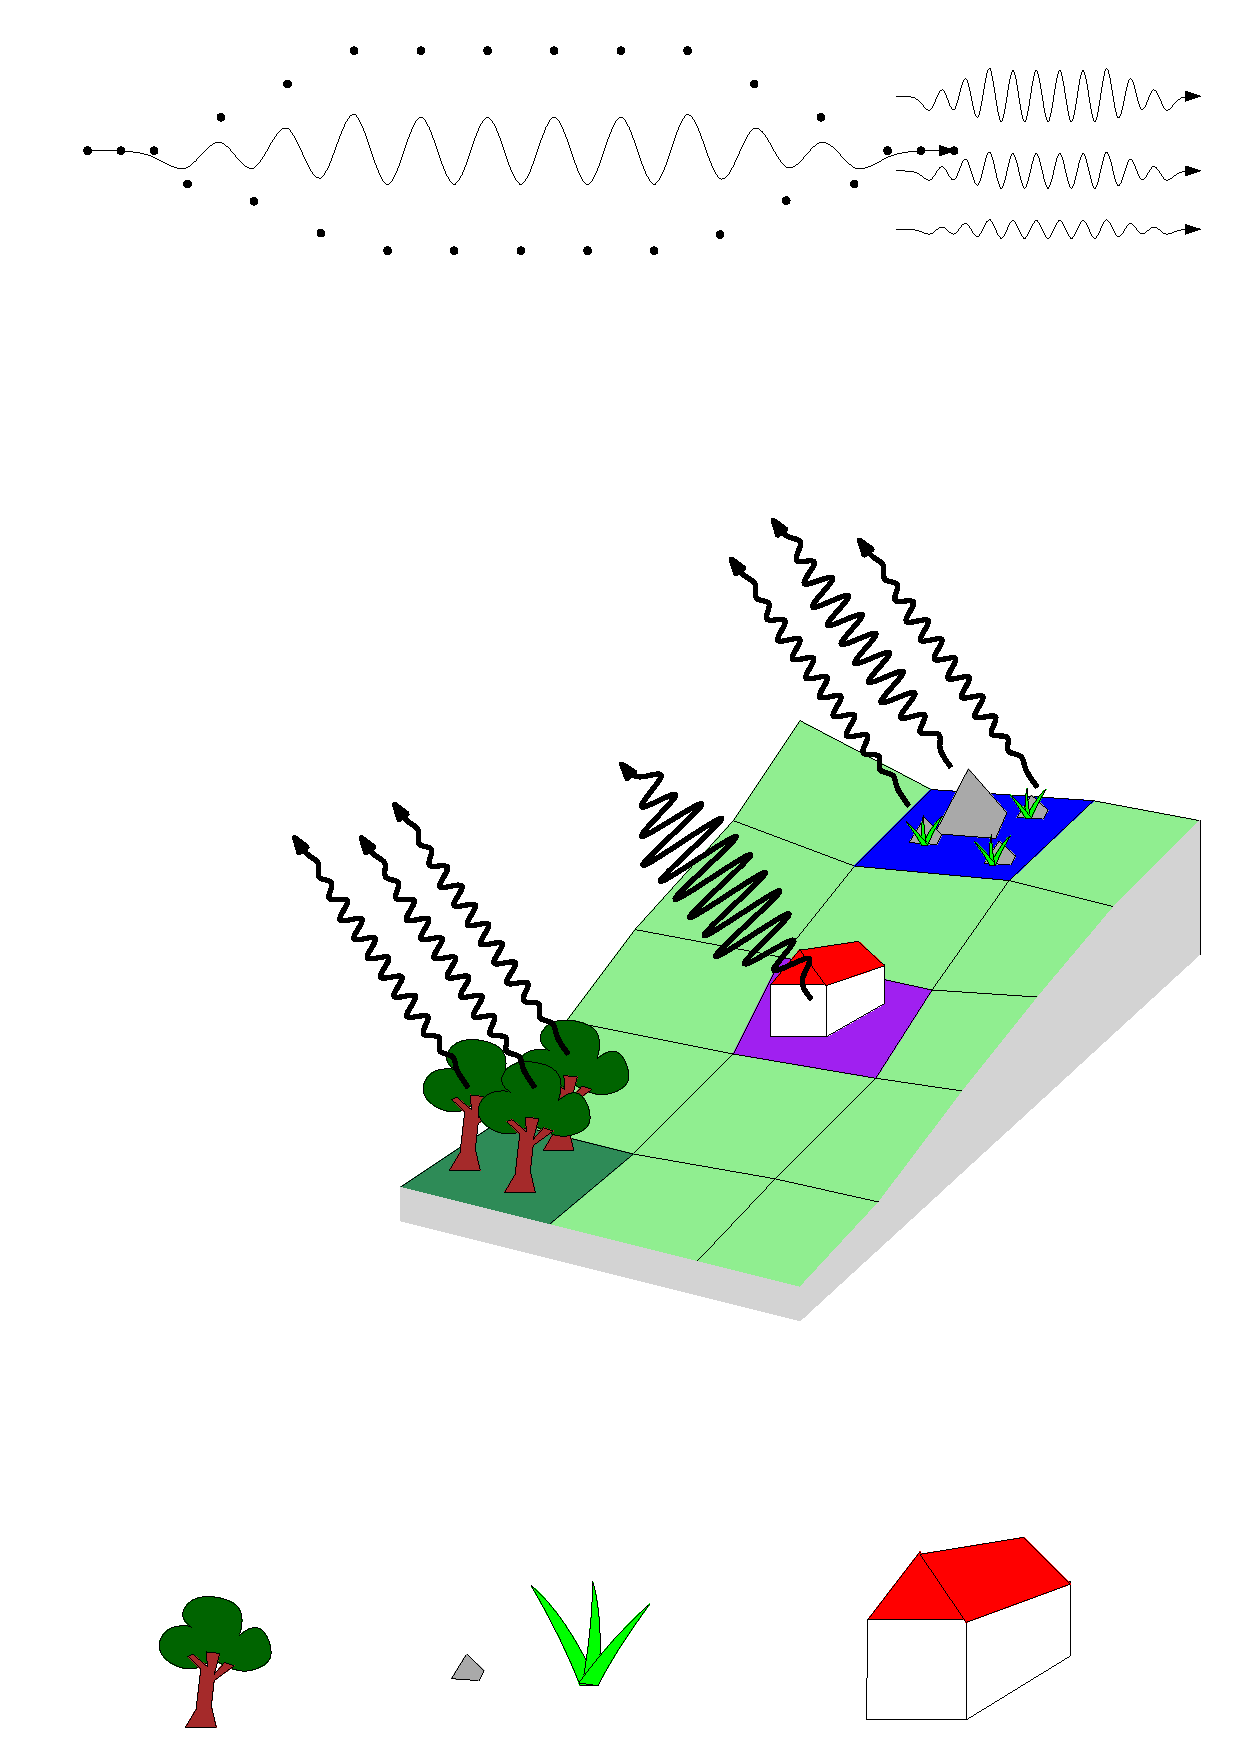
\includegraphics[width=0.45\linewidth,trim={2cm 6cm 0cm 8cm},clip]{figures/example1/figure} %  trim={<left> <lower> <right> <upper>}
	\fbox{
		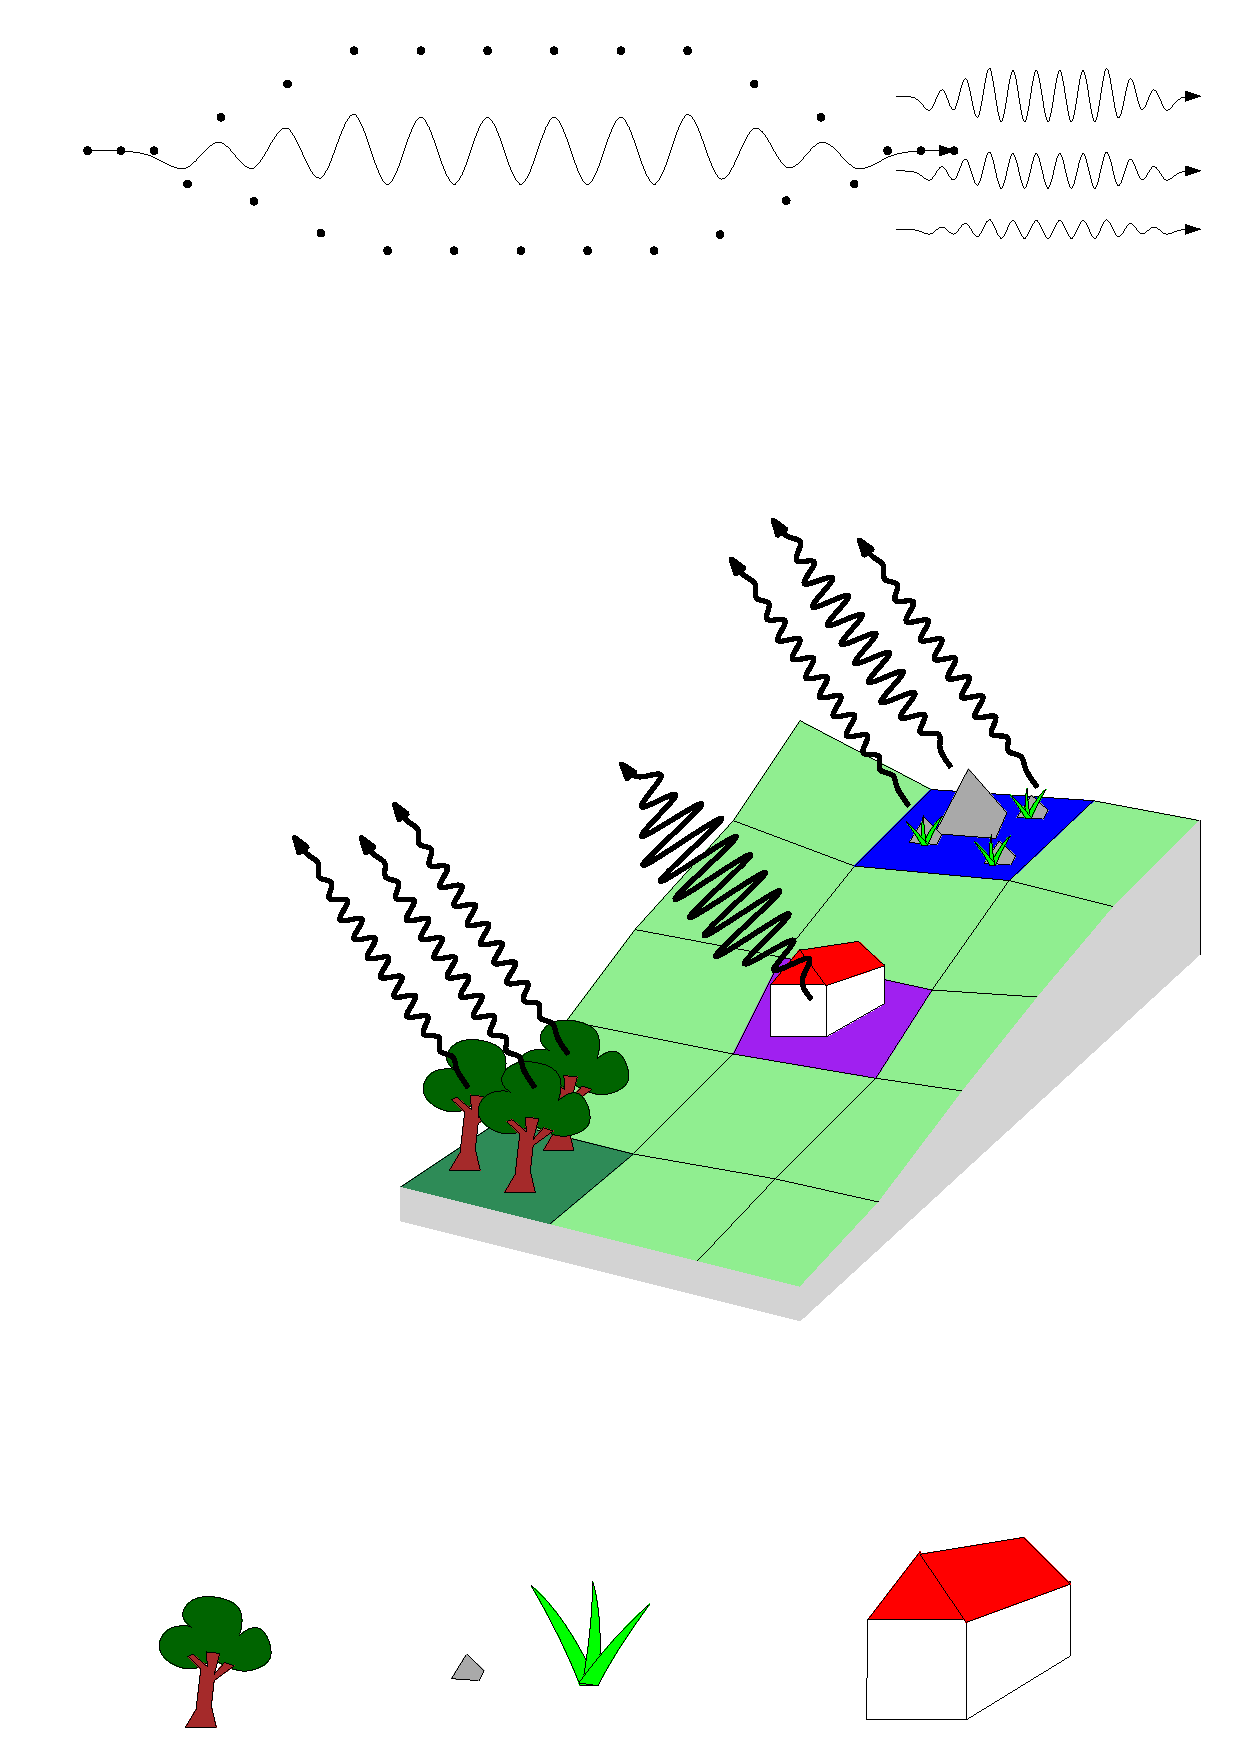
\includegraphics[width=0.45\linewidth,trim={2cm 6cm 0cm 8cm},clip]{figures/example1/figure} }%  trim={<left> <lower> <right> <upper>} 
	\caption{Double, including frame}
	\label{fig:double_example1}
\end{figure}



\begin{figure}[ht]
	\begin{subfigure}{.5\textwidth}
		\centering
		% include first image
	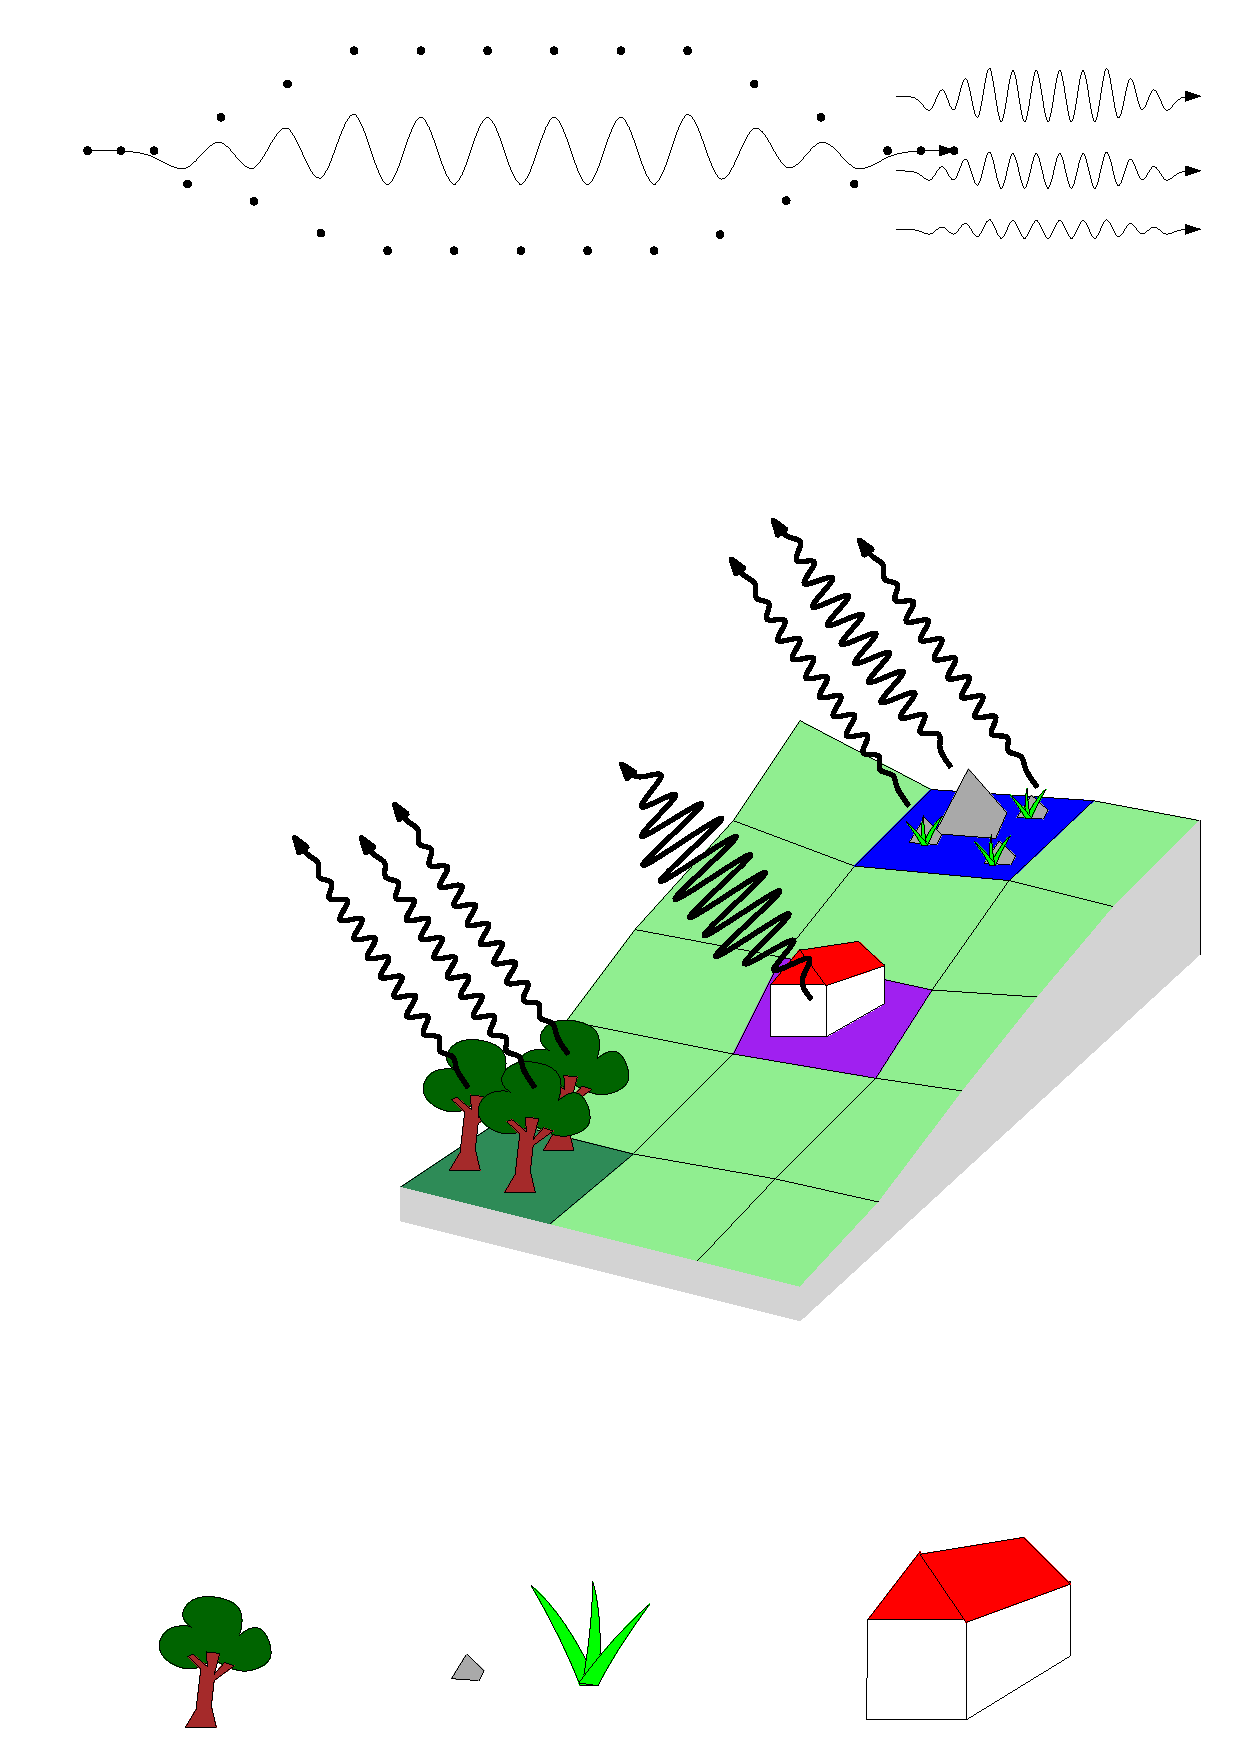
\includegraphics[width=1\linewidth,trim={2cm 6cm 0cm 8cm},clip]{figures/example1/figure} %  trim={<left> <lower> <right> <upper>}	
		\caption{Put your sub-caption here}
		\label{fig:sub-first}
	\end{subfigure}
	\begin{subfigure}{.5\textwidth}
		\centering
		% include second image
	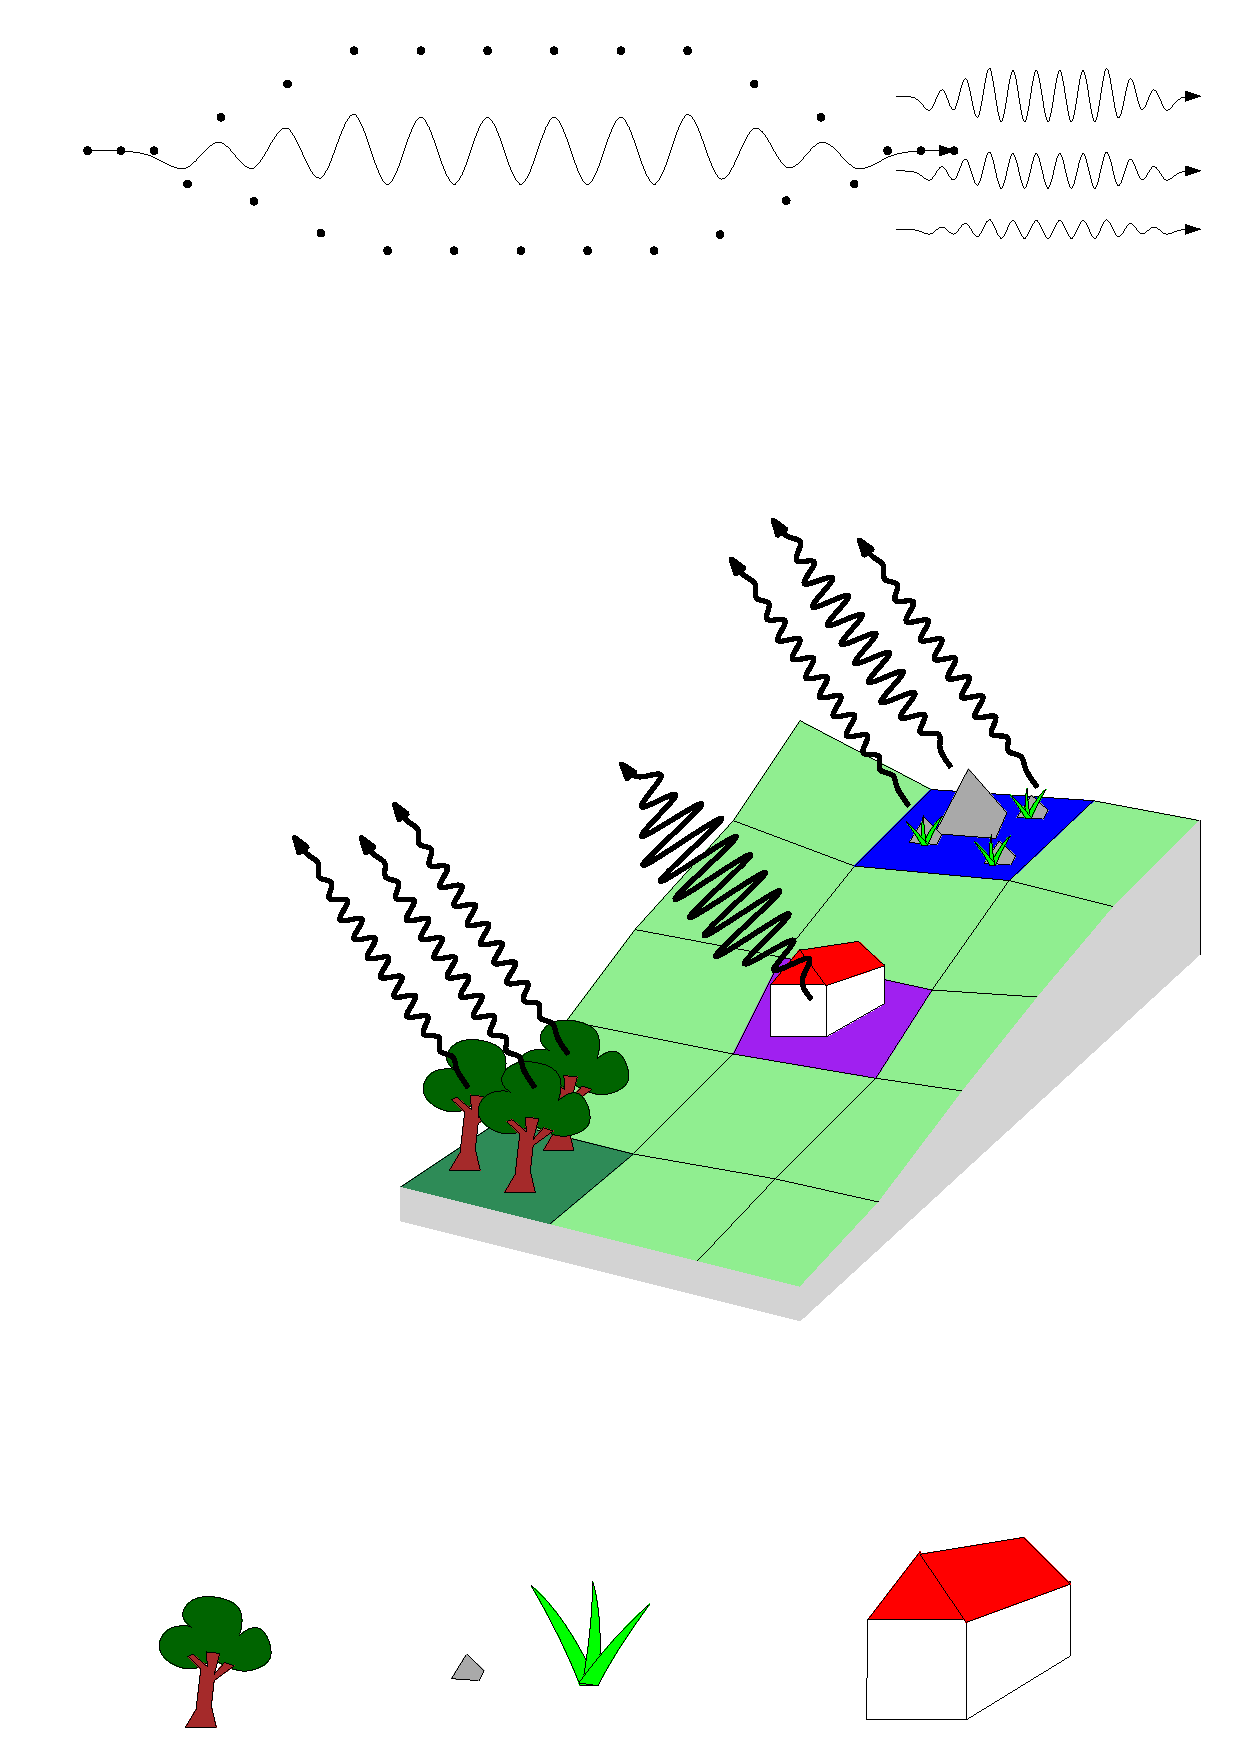
\includegraphics[width=1\linewidth,trim={2cm 6cm 0cm 8cm},clip]{figures/example1/figure} %  trim={<left> <lower> <right> <upper>}	
		\caption{Put your sub-caption here}
		\label{fig:sub-second}
	\end{subfigure}
	\caption{Put your caption here}
	\label{fig:fig}
\end{figure}

\begin{figure}[!hb]
	\centering
	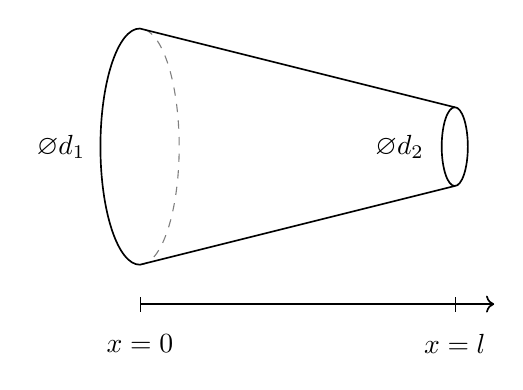
\begin{tikzpicture}
	\draw[dashed,color=gray] (0,0) arc (-90:90:0.5 and 1.5);% right half of the left ellipse
	\draw[semithick] (0,0) -- (4,1);% bottom line
	\draw[semithick] (0,3) -- (4,2);% top line
	\draw[semithick] (0,0) arc (270:90:0.5 and 1.5);% left half of the left ellipse
	\draw[semithick] (4,1.5) ellipse (0.166 and 0.5);% right ellipse
	\draw (-1,1.5) node {$\varnothing d_1$};
	\draw (3.3,1.5) node {$\varnothing d_2$};
	\draw[|-,semithick] (0,-0.5) -- (4,-0.5);
	\draw[|->,semithick] (4,-0.5) -- (4.5,-0.5);
	\draw (0,-1) node {$x=0$};
	\draw (4,-1) node {$x=l$};
	\end{tikzpicture}
	\caption{TikZ example: The graphic shows a truncated cone. The diameter of the cone changes from $d_1$ to $d_2$ along the x-direction.}
	\label{fig:exampletikz}
\end{figure}
\subsection{Referencing Figures}
Reference a Figure, the number will be CHAPTER.NUMFIG Figure \ref{fig:single_example1}
\begin{figure}[!b]
	\centering 
	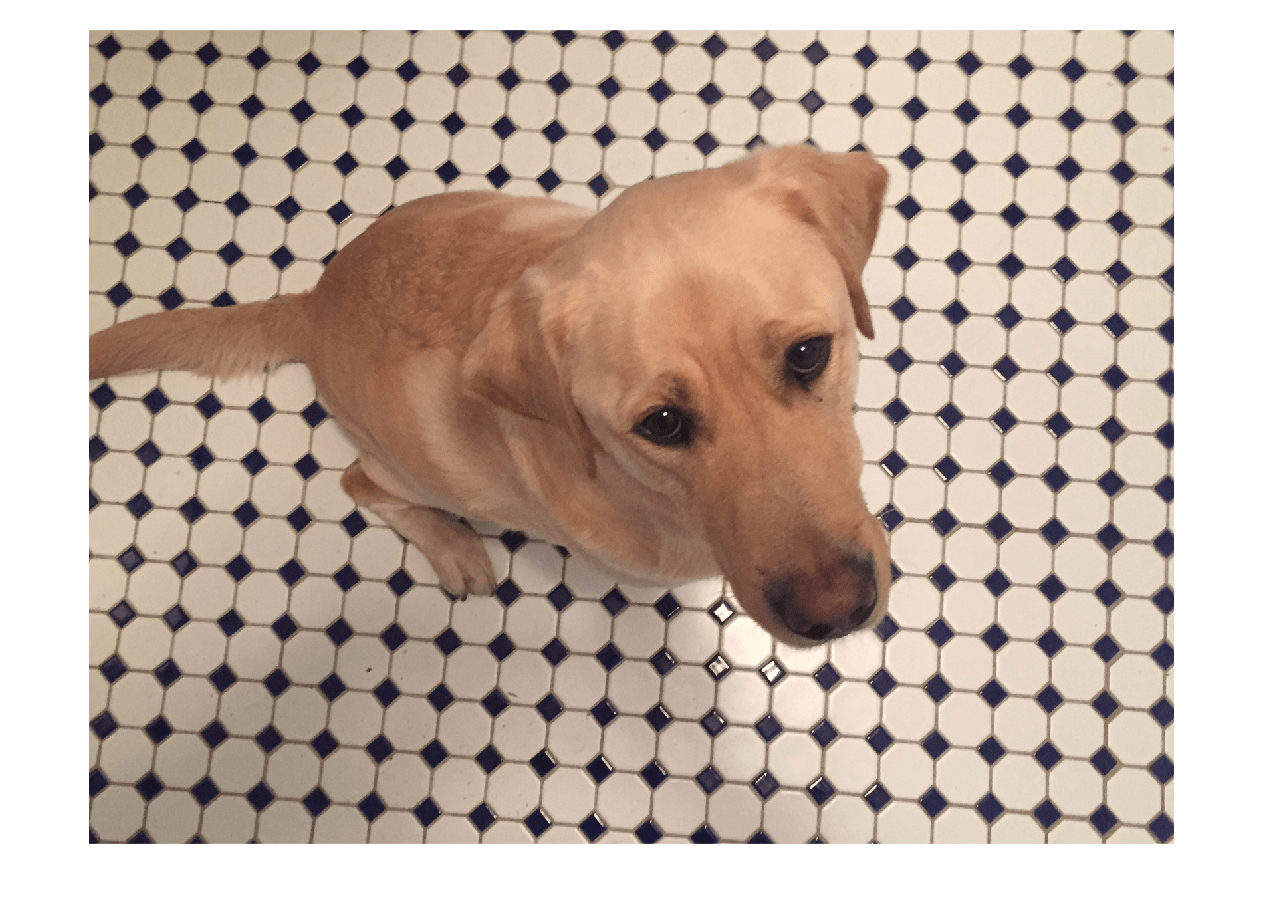
\includegraphics[width=0.7\linewidth,trim={2cm 6cm 0cm 8cm},clip,, angle =42 ]{figures/example2/figure} %  trim={<left> <lower> <right> <upper>}
	\caption{You can Rotated and crop an image in-line}
	\label{fig:single_example1}
\end{figure}


\FloatBarrier


\FloatBarrier

%%% Cahpter 2
%% Chapter 2
\chapter{Chapter}
\blindtext
\section{Section}
\blindtext
\section{Section}
\blindtext
\subsection{Subsection}
\blindtext
\paragraph{Paragraph}
\FloatBarrier

%%% Cahpter 3
%% Chapter 3
\chapter{Chapter}
\blindtext
\section{Section}
\blindtext
\section{Section}
\blindtext
\subsection{Subsection}
\blindtext
\paragraph{Paragraph}
\blindtext
\FloatBarrier

%%% Conclusion
\chapter{Conclusion and Outlook}

\blindtext

\blindtext

\blindtext

\blindtext

%%% Appendix


\appendix
\addcontentsline{toc}{chapter}{\protect\numberline{}Appendix}
\renewcommand{\thesection}{\Alph{section}}

\chapter*{Appendix}
\section{Publications}
\subsection{Pub 1}

\subsection{Pub 2}

\subsection{Pub 3}

\section{More}
\subsection{Ex }

\subsection{Pre}

\subsection{Post}

\section{Less}
\subsection{Ex }

\subsection{Pre}

\subsection{Post}





%\nociteMyPublicationsA{*}
%\bibliographyMyPublicationsA{MyPublicationsA}
%\bibentry{SchmohlSoergel2019}


{
\small
\bibliographystyle{apalike}   % 
\addcontentsline{toc}{chapter}{\protect\numberline{}Bibliography}
\bibliography{my_bibliography} % change for your .bib file


\normalsize
}

%%% Acknowledgements
\cleardoublepage
\thispagestyle{empty}


\chapter*{Acknowledgments} \addcontentsline{toc}{chapter}{\protect\numberline{}Acknowledgments}

There is a new trend among authors to thank every famous person for inspiration, non-existent assistance, and/or some casual reference to the author’s work. Authors do this to pump themselves up. So, on the off chance that this is helpful, I wish to thank the following people: 

The Emperor of Japan and the Queen of England for promoting literacy; William S. Cohen, former secretary of defense, for dropping me a note saying he liked my books, as did his boss, Bill Clinton; Bruce Willis, who called me one day and said, “Hey, you’re a good writer”; Albert Einstein, who inspired me to write about nuclear weapons; General George Armstrong Custer, whose brashness at the Little Bighorn taught me a lesson on judgement; Mikhail Gorbachev, whose courageous actions indirectly led to my books being translated into Russian; Don DeLillo and Joan Didion, whose books are always before and after mine on bookshelves, and whose names always appear before and after mine in almanacs and many lists of American writers—thanks for being there, guys; Julius Caesar, for showing the world that illiterate barbarians can be beaten; Paris Hilton, whose family hotel chain carries my books in their gift shops; and last but not least, Albert II, King of the Belgians, who once waved to me in Brussels as the Royal Procession moved from the Palace to the Parliament Building, screwing up traffic for half an hour, thereby forcing me to kill time by thinking of a great plot to dethrone the King of the Belgians. 

There are many more people I could thank, but time, space, and modesty compel me to stop here.

%%% CV
\cleardoublepage
\thispagestyle{empty}

\chapter*{Curriculum Vitae} \addcontentsline{toc}{chapter}{\protect\numberline{}Curriculum Vitae}


\begin{table*}[htbp]
	\centering
	\begin{tabular}{ll}
		\hspace{-0.25cm}\Large{\textbf{Personal}} & \\
		\vspace{-0.25cm} & \\
		Name & Philip J. Fry\\
		Date of Birth & August 14, 1974\\
		Place of Birth &  Brooklyn, New York  \\
		\vspace*{0.5cm} & \\
		\hspace{-0.25cm}\Large{\textbf{Education}} & \\
		\vspace{-0.25cm} & \\
		2018 - 2022 & Doctoral studies, Faculty for Aerospace Engineering and Geodesy, University of Stuttgart \\
		2015 - 2017 & Master of Science, Geodesy and Geoinformatics, University of Stuttgart \\
		2011 - 2015 & Bachelor of Science, Geodesy and Geoinformatics, University of Stuttgart \\
		2001 - 2010 & Gymnasium Manhattan, NYC \\
		\vspace*{0.5cm}  & \\
		\hspace{-0.25cm}\Large{\textbf{Experience}} & \\
		\vspace{-0.25cm} & \\
		2018 - current & Research Associate, Institute for Photogrammetry, University of Stuttgart \\
		2016 - 2017 & Research Assistant, Institute for Photogrammetry, University of Stuttgart \\
		2012 - 2014 & Teaching and Research Assistant, Institute of Engineering Geodesy, University of Stuttgart \\
		2010 - 2011 & Working Student,  Planet Express Inc., NYC. \\
		\vspace*{0.5cm}  & \\
		\hspace{-0.25cm}\Large{\textbf{Awards}} & \\
		\vspace{-0.25cm} & \\
		2018 &  Robot Arms Apts Award for year’s best master thesis \\
		2016 &  Mars University Award for year’s best bachelor’s degree \\
	\end{tabular}
\end{table*}




\end{document}


